\section{A survey of matrix mappings}
In the following pages we will look at three different kinds of mappings for a matrix $\Acc{m}{n}$: no frustration, frustration in one direction, frustration in both directions.

There are two different ways to frustrate a mapping:
\begin{enumerate}
\item geometric deficiency - mapping into a higher dimension space;
\item algebraic deficiency - rank deficiency in row or column.
\end{enumerate}

These tables specify critical properties of the target matrix.

\textbf{Plots: }The plots show the image of the unit circle under the mapping action of the target matrix and its transpose. All plots start with the unit circle which is either
\begin{equation}
  \begin{array}{rcll}
     S(\theta) &=& \mat{c}{\cos \theta\\\sin \theta},\ \theta\in[0,2\pi) \qquad &n=2,\\
     S(\theta,\phi) &=& \mat{c}{\cos \theta\sin \phi\\\sin \theta \sin \phi\\\cos \phi},\ \theta\in[0,2\pi),\ \phi\in[0,\pi), \qquad &n=3.
  \end{array}
\end{equation}
Then look at the mapping action of the matrix. The result is either
\begin{equation}
  \A{}S(\theta) 
\end{equation}
when the target matrix has two columns or
\begin{equation}
  \A{}S(\theta,\phi) 
\end{equation}
when the target matrix has three columns.\\
%%
\textbf{Vector space mappings:}

\textbf{Matrix images:}

\textbf{Matrix ranks:}


\clearpage

%%
%% 2 x 2
%%
\begin{table}[htdp]
\begin{center}
\begin{tabular}{cc}
  $\A{}x=y$ & $\A{T}y=x$\\
 $\textellipsis$ & $\textellipsis$ \\
$\mat{rr}{1&2\\-1&2}\mat{c}{x_{1}\\x_{2}} = \mat{c}{y_{1}\\y_{2}}$ &
$\mat{rr}{1&-1\\2&2}\mat{c}{x_{1}\\x_{2}} = \mat{c}{y_{1}\\y_{2}}$ \\
\ \\
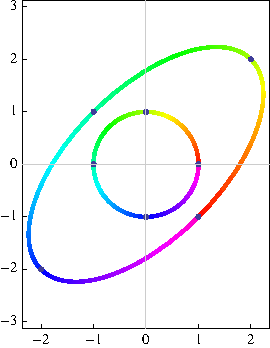
\includegraphics[ width = 2.15in ]{pdf/post_mortemII/2_2_2} &
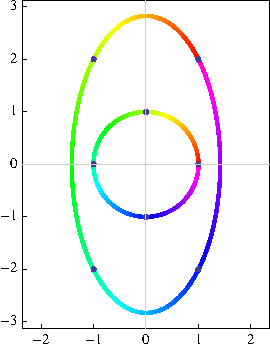
\includegraphics[ width = 2.15in ]{pdf/post_mortemII/2_2_2_t} \\
%%
\ \\
 matrix image & transpose matrix image \\
unit circle $\mapsto$ ellipse & unit circle $\mapsto$ ellipse\\
 $\textellipsis$ & $\textellipsis$ \\
vector space mappings & vector space mappings\\
(Domain) $\real{2} \mapsto \real{2}$ (Codomain) & (Codomain) $\real{2} \mapsto \real{2}$ (Domain)\\
 $\textellipsis$ & $\textellipsis$ \\
 full column rank  & full row rank\\[10pt]
\end{tabular}
\end{center}
\label{tab:interpII:a}
\caption{Maps with no frustration. The domain and the codomain have the same dimension and the matrix has full rank. There are no null spaces associated with either the matrix or its transpose.}
\end{table}%

boo hoo

\clearpage
%%
%% 2 x 3
%%
\begin{table}[htdp]
\begin{center}
\begin{tabular}{cc}
  $\A{}x=y$ & $\A{T}y=x$\\
 $\textellipsis$ & $\textellipsis$ \\
$\mat{ccc}{0&3&0\\1&1&2}\mat{c}{x_{1}\\x_{2}\\x_{3}} = \mat{c}{y_{1}\\y_{2}}$ &
$\mat{cc}{0&1\\3&1\\0&2}\mat{c}{y_{1}\\y_{2}} = \mat{c}{x_{1}\\x_{2}\\x_{3}}$ \\
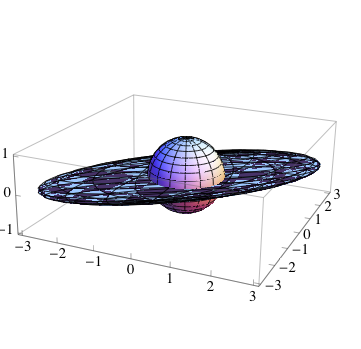
\includegraphics[ width = 2.5in ]{pdf/post_mortemII/3_2_2.png} &
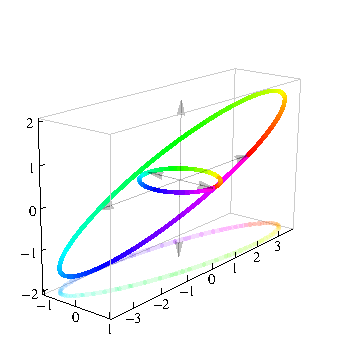
\includegraphics[ width = 2.5in ]{pdf/post_mortemII/3_2_2_t} \\
%%
vector space mappings & vector space mappings\\
(Domain) $\real{3} \mapsto \real{2}$ (Codomain) & (Codomain) $\real{2} \mapsto \real{3}$ (Domain)\\
 $\textellipsis$ & $\textellipsis$ \\
 matrix image & transpose matrix image \\
unit sphere $\mapsto$ elliptic disk & unit circle $\mapsto$ ellipse\\
 $\textellipsis$ & $\textellipsis$ \\
column rank deficient & full row rank\\[10pt]
\end{tabular}
\end{center}
\label{tab:interpII:a}
\caption{Frustration in one direction: domain to codomain. The frustration is signaled by the column rank deficiency. Such deficiencies arise in one of two ways: either there are more columns than rows $(n>m)$ or some column vectors are linearly dependent $(\rho<m)$.}
\end{table}

\clearpage
%%
%% 3 x 2
%%
\begin{table}[htdp]
\begin{center}
\begin{tabular}{cc}
  $\A{}x=y$ & $\A{T}y=x$\\
 $\textellipsis$ & $\textellipsis$ \\
$\Aexample \mat{c}{x_{1}\\x_{2}} = \mat{c}{y_{1}\\y_{2}\\y_{3}}$ &
$\Atexample\mat{c}{x_{1}\\x_{2}\\x_{3}} = \mat{c}{y_{1}\\y_{2}}$ \\
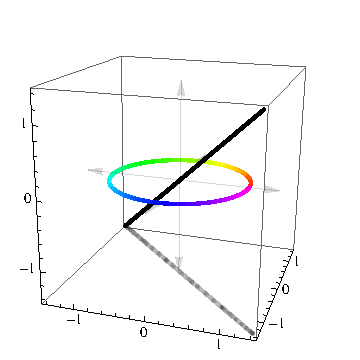
\includegraphics[ width = 2.5in ]{pdf/post_mortemII/3_2_1_a} &
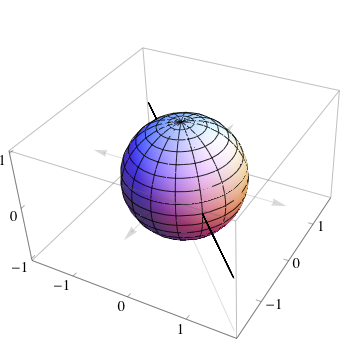
\includegraphics[ width = 2.5in ]{pdf/post_mortemII/3_2_1_t_a} \\
%%
vector space mappings & vector space mappings\\
(Domain) $\real{2} \mapsto \real{3}$ (Codomain) & (Codomain) $\real{3} \mapsto \real{2}$ (Domain)\\
 $\textellipsis$ & $\textellipsis$ \\
 matrix image & transpose matrix image \\
unit circle $\mapsto$ line & unit sphere $\mapsto$ line\\
 $\textellipsis$ & $\textellipsis$ \\
column rank deficient & row rank deficient\\[10pt]
\end{tabular}
\end{center}
\label{tab:interpII:c}
\caption{Frustration in both direction: domain to codomain. The frustration is signaled by the column rank deficiency. Such deficiencies arise in one of two ways: either there are more columns than rows $(n>m)$ or some column vectors are linearly dependent $(\rho<m)$.}
\end{table}

\endinput
